\documentclass{hw}
\usepackage{mhchem}
\usepackage{nuc}
\usepackage{siunitx}
\usepackage{amsmath}
\usepackage{cancel}
\usepackage{physics}
\usepackage{booktabs}
\graphicspath{ {images/}}

\DeclareSIUnit\eVperc{\eV\per c^2}
\DeclareSIUnit\curie{Ci}
\DeclareSIUnit\roentgen{R}
\DeclareSIUnit\week{wk}
\DeclareSIUnit\year{yr}

\author{J.R. Powers-Luhn}
\date{2016/12/8}
\title{NE551 Final Exam}

\begin{document}

\problem{}
A flux of \SI{100}{\electronvolt} neutrons 
(\SI{1e9}{neutrons \per\centi\meter^2\per\second}) is incident on a \ce{^{197}Au} disk 
that is \SI{1}{\centi\meter} in diameter and is \SI{2.54e-3}{\centi\meter} thick.
\begin{enumerate}
    \item Calculate the absorption cross section using a thermal cross section 
    of \SI{98.7}{\barn}. Compare with the \SI{100}{\electronvolt} absorption 
    cross section from the NNDC ENDF/B-VII.1 evaluation and explain why the two 
    values are different.
    \item Calculate the Q-value for the absorption reaction: \ce{n+^{197}Au 
    \rightarrow ^{198}Au} (mass excesses are: 
    $\mathrm{n}$=\SI{8.071}{\mega\eVperc}, 
    \ce{^{197}Au}=\SI{-31.141}{\mega\eVperc}, 
    \ce{^{198}Au}=\SI{-29.582}{\mega\eVperc}).
    \item The kinetic energy of the \ce{^{198}Au} immediately after the 
    absorption of the neutron and before the emission of any gamma rays from 
    the compound \ce{^{198}Au} nucleus.
    \item The activity of \ce{^{198}Au} after 7 days of irradiation. Use the 
    NNDC ENDF/B-VII.1 value of the absorption cross section at 
    \SI{100}{\electronvolt}.
\end{enumerate}

\solution
\part
For low energies, $\sigma_a \propto v^{-1} \propto \sqrt{\frac{1}{T}}$.

\begin{align*}
    \sigma_a \left( E \right) &\approx \sigma_a^{Th} \sqrt{\frac{E_{Th}}{E}} \\
    &\approx \SI{98.7}{\barn} \sqrt{\frac{\SI{0.025}{\electronvolt}}
    {\SI{100}{\electronvolt}}} \\
    &\approx \SI{1.56}{\barn} 
\end{align*}

From NNDC ENDF/B-VII.1 we use the values of (\SI{100.246}{\electronvolt}, 
\SI{3.99648}{\barn}) and (\SI{99.579}{\electronvolt}, \SI{3.90669}{\barn}) to 
interpolate and arrive at a value of \SI{3.96336}{\barn}. This is much larger 
than the calculated value. From the plot of cross sections (figure 
\ref{fig:197AuCrossSection}) we see that at this point we have entered the 
resonance region for this nucleus. Since the A number is relatively high for 
gold, there are many available energy states--and the resonance region starts 
at comparatively low energies.

\begin{figure}[h]
    \begin{centering}
	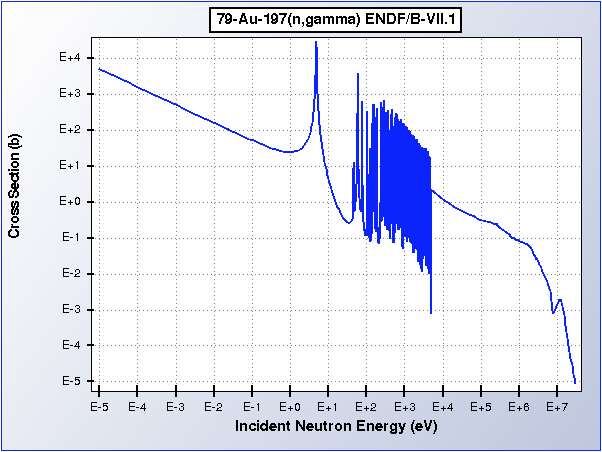
\includegraphics[width=10cm,height=10cm,keepaspectratio]{197AuCrossSection}
	\caption{Absorption cross section for \ce{^{197}Au}}
	\label{fig:197AuCrossSection}
    \end{centering}
\end{figure}

\part
\begin{align*}
    Q &= \left( M_X + M_\neutron - M_Y \right) c^2 \\
    \intertext{Use mass excess in lieu of mass}
    &= \SI{-31.141}{\mega\electronvolt} + \SI{8.071}{\mega\electronvolt} - 
    \SI{-29.582}{\mega\electronvolt} \\
    &= \SI{6.512}{\mega\electronvolt}
\end{align*}

\part
Since the incident neutron energy is much less than its mass, we can ignore 
relativistic effects and calculate the kinetic energy of the \ce{^{198}Au} 
using conservation of momentum.

\begin{align*}
    \sqrt{2 m_{\neutron} E_{\neutron}} &= 
    \sqrt{2 m_{\ce{^{198}Au}} E_{\ce{^{198}Au}} } \\
    E_{\ce{^{198}Au}} &= E_{\neutron} \frac{m_{\neutron}}{m_{\ce{^{198}Au}}} \\
    &= \SI{100}{\electronvolt} \frac{\SI{1.00866}{\amu}}{\SI{197.968}{\amu}} \\
    &= \SI{0.510}{\mega\electronvolt}
\end{align*}

\part
Since NNDC gives no cross section for \ce{^{198}Au}, assume it does not absorb 
neutrons.

\begin{align*}
    \dot{N}_{197} &= -N_{197} \sigma_a \phi \\
    \dot{N}_{198} &= N_{197} \sigma_a \phi - \lambda_{198} N_{198}
\end{align*}

Solving these gives:

\begin{align*}
    A(t) &= N_{197} \sigma_a \phi \left( 1 - \exp{-\lambda t} \right) \\
    N_{197} &= \frac{A_V}{m_{197}} m_{Au} \\
    m_{Au} &= \rho V = \rho \times \pi (\SI{0.5}{\centi\meter})^2 
    \left(\SI{2.54e-3}{\centi\meter}\right) = 
    \SI{19.32}{\gram\per\centi\meter^3} \times \SI{1.96e-3}{\centi\meter^3} \\
    &= \SI{3.79e-2}{\gram} \\
    N_{197} &= \frac{\num{6.022e23}}{\SI{196.966}{\gram}}\SI{3.79e-2}{\gram} = 
    \num{1.16e20}\\
    \lambda &= \frac{\log{2}}{\SI{2.69517}{\day}} = \SI{0.2572}{\per\day} \\
    A(\SI{7}{\day}) &= \num{1.16e20} \times 
    \SI{3.96336e-24}{\per\centi\meter^2} \times 
    \SI{1e9}{neutrons \per \centi\meter^2} \times
    \left( 1 - \exp{- \SI{0.2572}{\per\day} \times \SI{7}{\day}} \right) \\
    &= \SI{3.84e5}{\becquerel}
\end{align*}

\problem{}
A beam of \SI{1}{\mega\electronvolt} neutrons is incident upon a \ce{^{12}C} 
graphite target, density=\SI{2.2}{\gram\per\centi\meter^3}. Using the CENDL 
elastic scattering cross section, determine the mass-energy transfer 
coefficient for \SI{1}{\mega\electronvolt} \ce{n + ^{12}C} s-wave elastic 
scattering, assuming all of the scattering is elastic at this energy.

\solution
Anderson equation 8.45:
\begin{align*}
    \left(\frac{\mu_{tr}}{\rho}\right)_{es} &= 
    \left(\frac{\mu}{\rho}\right)_{es} 
    \left[ \frac{\left<T_A\right>}{T} \right] \\
    &= \left(\frac{\mu}{\rho}\right)_{es}
    \left[ \frac{T - \left<T^\prime\right>}{T} \right] \\
    \left(\frac{\mu}{\rho}\right)_{es} &= n_m \sigma_{es}
\end{align*}

From CENDL, $\sigma_{es}=\SI{2.49078}{\barn}$

\begin{align*}
    \left(\frac{\mu_{tr}}{\rho}\right)_{es} &=
    n_m \sigma_{es} \left[ \frac{1-\alpha}{2} \right] \\
    \alpha &= \left[ \frac{A-1}{A+1} \right]^2 \approx 0.716 \\
    \left(\frac{\mu_{tr}}{\rho}\right)_{es} &= 
    \frac{\rho A_V}{m_m} \sigma_{es} \left[ \frac{1-\alpha}{2} \right] \\
    &= \frac{\SI{2.2}{\gram\per\centi\meter^3} \times \num{6.022e23}}
    {\SI{12}{\gram}} \times \SI{2.49078e-24}{\centi\meter^2} \times 
    \left[ \frac{1-\num{0.716}}{2} \right] \\
    &= \SI{0.039}{\per\centi\meter}
\end{align*}

\problem{}
Define what is meant by stochastic biological effects due to radiation and list 
two such effects in humans.

\solution
Stochastic biological effects are effects from radiation which grow more likely 
as exposure increases, but do not become more severe. The symptoms may occur 
long after the exposure. Any radiation exposure increases the probability of 
occurence (according to the linear-no-threshold theory), which leads to the 
ALARA principle. Two examples are solid tumor formation and leukemia.

\problem{}
Define what is meant by deterministic biological effects due to radiation and 
list two such effects in humans.

\solution
Deterministic effects are a direct result of damage from the radiation 
exposure. The severity of the effects increases with the amount of exposure, 
and different effects occur at different minimum threshold levels. Examples 
include hair loss and nausea/vomiting.

\problem{}
Explain the importance of cell cycle in regards to the deleterious biological 
effects from radiation.

\solution
Different cells divide at different rates. Since the ongoing biological damage 
(stochastic effects) depends on damage to cell DNA being propogated through 
cell generations, the time relative to that cell dividing is relevant to the 
resultant damage. If the cell has just been born, DNA damage is likely to be 
repaired or detected before the cell can reproduce, preventing the propogation 
of the mutation/damage. If the cell is damaged just before it reproduces, 
then that alteration is more likely to spread to its daughter cells before 
it can be repaired.

\problem{}
A \SI{144}{\curie} point source of \ce{^{24}Na} is to be stored at the bottom 
of a pool of water. \ce{^{24}Na} decays by beta emission to stable 
\ce{^{24}Mg}. In the decay process it emits two gammas per disintegration with 
energies \SI{2.75}{\mega\electronvolt} and \SI{1.37}{\mega\electronvolt}. How 
deep must the water be if the exposure rate at a point \SI{6}{\meter} above the 
source is not to exceed \SI{20}{\milli\roentgen\per\hour}?

\solution
Assume that for these photon energies, the dose rate equation 
\ref{eqn:unshielded} is valid to calculate unshielded dose. From Turner figure 
8.9, we find that the mass attenuation coefficients are 
\SI{0.043}{\per\centi\meter} ($\gamma_1$) and \SI{0.061}{\per\centi\meter} 
($\gamma_2$). First we focus on $\gamma_1$.

\begin{equation*}
    \label{eqn:unshielded}
    \dot{X} = \frac{0.5 \times C \times E}{r^2} \numberthis
\end{equation*}

Equation \ref{eqn:unshielded} gives an exposure of 
\SI{5500}{\milli\roentgen\per\hour}. To determine the shielding needed to reduce this 
to \SI{20}{\milli\roentgen\per\hour}, we use equation \ref{eqn:shielding} to 
arrive at \num{5.62}. This does not account for the buildup factor, so we must 
interpolate from Turner figure 15.2 to deterimine $B_1^{(1)} \approx 5.8$. To 
shield against this additional factor we calculate $\left(\mu t\right)^{(1)} 
= \left(\mu t\right)^{(0)} + \log{B_1^{(1)}} \approx \num{7.41}$. Repeating 
this process iteratively, we arrive at a final buildup factor of \num{7.62}.

\begin{align*}
    \label{eqn:shielding}
    \dot{X}_{shielded} &= \dot{X}_{unshielded} \mathrm{e}^{-\mu t} \numberthis \\
    \SI{20}{\milli\roentgen\per\hour} &= \SI{5500}{\milli\roentgen\per\hour} 
    \mathrm{e}^{-\mu t} \\
    \mu t &= 5.62
\end{align*}

We then multiply equation \ref{eqn:shielding} by this factor to determine a 
value given that $\mu_1 t = 7.65$:

\begin{align*}
    \dot{X}_{shielded} &= 7.62 \times 5500 \times \mathrm{e}^{-7.65} \\
    &= 19.93
\end{align*}

Next we determine, given this shielding, the dose contribution from the 
\SI{1.37}{\mega\electronvolt} gamma.

\begin{align*}
    \mu_2 t &= \mu_1 t \times \frac{E_2}{E_1} \\
    &= 7.65 \times \frac{0.061}{0.043} \\
    &= 10.85
\end{align*}

This is off of figure 15.2, so instead I interpolated in the tables found at 
\url{http://www.nucleonica.net/Application/Help/Helpfiles/Appendix4.htm}. 
Not following the same iterative procedure as before (since $\mu t$ is now 
fixed), I arrived at a buildup factor of \num{21.54} (see attached code). This 
resulted in a dose contribution of \SI{0.0011}{\milli\roentgen\per\hour}

\begin{align*}
    \dot{X}_{sh} &= \num{21.54} \times \frac{0.5 \times \SI{144}{\curie} \times 
    \SI{1.37}{\mega\electronvolt}}{\SI{6}{\meter}^2} \times 
    \mathrm{e}^{-10.85} \\
    &= \SI{0.0011}{\milli\roentgen\per\hour}
\end{align*}

This gives a total exposure rate of \SI{19.93}{\milli\roentgen\per\hour}. To 
determine the thickness of water, then, we use $\mu t / \mu = \num{7.65} / 
\SI{0.043}{\per\centi\meter} = \SI{177.9}{\centi\meter}$

\problem{}
Calculate the whole body effective dose for an individual who has 
simultaneously received all of the following exposures:
\begin{enumerate}
    \item \SI{2}{\milli\gray} alpha to the lung
    \item \SI{5}{\milli\gray} thermal neutrons to the whole body
    \item \SI{5}{\milli\gray} gamma, whole body
    \item \SI{40}{\milli\gray} beta to the thyroid
    \item \SI{2}{\gray} beta to the skin
\end{enumerate}

Which, if any, of the recommended annual exposure limits from NCRP 116 (see 
\url{https://www.ceessentials.net/article6#section5_5}) for occupational 
exposures are exceeded?

\solution
To determine dose we use equation \ref{eqn:dose}, where $D$ is the 
exposure and $Q$ is the quality factor for the radiation in question. For 
quality factors we refer to the ICRP 103 specifications 
(\url{https://www.euronuclear.org/info/encyclopedia/r/radiation-weight-factor.htm}) 
and arrive at 1 for betas and photons, 20 for alphas, and 2.5 for thermal 
neutrons (calculated using equation \ref{eqn:q_neutron}).

\begin{equation*}
    \label{eqn:dose}
    H_T = Q \times D \numberthis
\end{equation*}

\begin{equation*}
    \label{eqn:q_neutron}
    Q(E) = 2.5 + 18.2 \mathrm{e}^{-\left[ \log(E) \right]^2 / 6} \numberthis
\end{equation*}

To convert this value into a whole body dose equivalent, we use equation 
\ref{eqn:wbde} which uses a tissue weighting factor to convert dose applied to 
a specific organ into the dose to the whole body that would cause the 
equivalent stochastic biological damage. Tissue weighting factors were obtained 
from the 2007 ICRP report, accessed from 
\url{http://www.icrp.org/docs/David%20Brenner%20Effective%20Dose%20a%20Flawed%20Concept.pdf}. 
The values used were 0.12 for lungs, 0.04 for thyroid, and 0.01 for skin.

\begin{equation*}
    \label{eqn:wbde}
    E = \sum_T w_T H_T \numberthis
\end{equation*}

\begin{tabular}{rllrr}
\toprule
Exposure (mGy) &        Radiation &      Target &    Dose &  Whole-Body Equivalent \\
\midrule
             2 &            alpha &        lung &    40.0 &                    4.8 \\
             5 &  thermal neutron &  whole body &    12.5 &                   12.5 \\
             5 &            gamma &  whole body &     5.0 &                    5.0 \\
            40 &             beta &     thyroid &    40.0 &                    1.6 \\
          2000 &             beta &        skin &  2000.0 &                   20.0 \\
\bottomrule
\end{tabular}

The total dose was determined to be \SI{43.9}{\milli\gray}. This does not 
exceed the NRCP 116 annual exposure limit of \SI{50}{\milli\gray} per year, nor 
does it exceed the dose limit to the skin. Assuming that the worker is an 
adult, lifetime dose limits are also likely not a problem. That said, it is 
possible that local control limits may have been violated.

\problem{}
Suppose that a \SI{1}{\milli\curie} soft beta emitter is distributed uniformly 
through your body. Calculate 
\begin{enumerate}
    \item the effective dose after 1 year, 
    \item the effective dose after 5 years, and 
    \item the committed effective doses 
\end{enumerate}
for an occupational worker based on the following:
\begin{itemize}
    \item The physical half life is 2 years and the biological half life is 1 
    year
    \item The energy deposited per decay is \SI{10}{\kilo\electronvolt}
    \item The body has a mass of \SI{74}{\kilo\gram}
\end{itemize}

\solution
Dose as a function of time can be calculated using equation 
\ref{eqn:dose_of_time}. In this case, since the energy deposited per decay is 
given, we know that $w=\SI{10}{\kilo\electronvolt}$. We also assume that all 
energy is contained in the body, so $\phi_{af}=1$.

\begin{equation*}
    \label{eqn:dose_of_time}
    D(t) = \frac{C_{max} \Delta}{\left(\lambda_p + \lambda_b \right)} 
    \phi_{af} \left[ 1 - \mathrm{e}^{-\left(\lambda_p + \lambda_b \right) t} 
    \right] \numberthis \\
\end{equation*}

\part
$$D(\SI{1}{\year}) = \frac{\SI{5e5}{\becquerel\per\kilo\gram} \times \SI{1.6e-15}{\joule\per decay}}{\SI{3.29e-8}{\per\second}}
\times \mathrm{e}^{-\SI{3.29e8}{\per\second} \times \SI{3.16e7}{\second}} = \SI{15.7}{\milli\sievert}$$

\part
$$D(\SI{5}{\year}) = \frac{\SI{5e5}{\becquerel\per\kilo\gram} \times \SI{1.6e-15}{\joule\per decay}}{\SI{3.29e-8}{\per\second}}
\times \mathrm{e}^{-\SI{3.29e8}{\per\second} \times 5 \times \SI{3.16e7}{\second}} = \SI{24.1}{\milli\sievert}$$

\part
$$ CDE = \frac{\SI{5e5}{\becquerel\per\kilo\gram} \times \SI{1.6e-15}{\joule\per decay}}{\SI{3.29e-8}{\per\second}} = 
\SI{24.3}{\milli\sievert}$$

\problem{}
Using the BULK II tool discussed in class, calculate the thickness of concrete 
shielding needed to reduce the dose at points A, B, and C to 
\SI{100}{\milli\sievert} in a year for a worker standing \SI{50}{\centi\meter} 
away from the outside of the concrete shielding. Assume the worker is there 20 
hours per week, and works 40 weeks per year treating patients. The distance 
from the target (patient) center to the concrete walls is 
\SI{250}{\centi\meter} in the +Y direction, \SI{200}{\centi\meter} in the -Y 
direction, \SI{250}{\centi\meter} in the +X direction, \SI{200}{\centi\meter} 
in the -X direction, \SI{250}{\centi\meter} in the +Z direction, and 
\SI{100}{\centi\meter} in the -Z direction, with the target defining isocenter. 
Use a density of \num{2.3} for the concrete. Use water for the target. Beam 
moves along the y-axis in the +Y direction. Points A, B, C lie in the Z=0 
plane. Design the shielding for \SI{230}{\mega\electronvolt} proton facility 
with a beam current of \SI{10}{\nano\ampere} (\SI{1e-8}{\coulomb\per\second}) 
on target. Either copy the input and output tabs from your results, or email 
the entire work book along with the rest of your exam.

\solution
The allowed exposure per week is $\SI{100}{\milli\sievert\per\year} / 
\SI{40}{\week\per\year} = \SI{2.5}{\milli\sievert\per\week} = 
\SI{2.5e3}{\micro\sievert\per\week}$

A spreadsheet is included in this email with final values. The +X wall is 
\SI{106}{\centi\meter} thick; the -X wall is \SI{114}{\centi\meter} thick; and 
the +Y wall is \SI{291}{\centi\meter} thick. This gave final exposure values of 
\SI{2.45}{\milli\sievert\per\week}, \SI{2.43}{\milli\sievert\per\week}, and 
\SI{2.37}{\milli\sievert\per\week} at points A, B, and C respectively.

\end{document}